\documentclass[lang=cn,11pt,a4paper,cite=authornum]{paper}

\title{大数据技术基础 实验三 \\ 实验报告}
\author{毛子恒 \\ 2019211397}
\institute{北京邮电大学\ 计算机学院}

\date{\zhtoday}

% 本文档命令
\nocite{*}

\begin{document}

\maketitle

\section{概述}

\subsection{实验目的}

掌握HBase、ZooKeeper的安装与使用,使用MapReduce批量将HBase表上的数据导入到HDFS中,学习本实验能快速掌握HBase数据库在分布式计算中的应用,理解Java API读取HBase数据等相关内容。

\subsection{实验步骤}

\begin{enumerate}
    \item 下载安装并配置Zookeeper;
    \item 下载并安装HBase;
    \item HBase实践。
\end{enumerate}

\section{实验结果及分析}

\paragraph{HBase Shell实践}

进入HBase Shell,输入命令,创建名为\mintinline{text}{2019211397-mzh}的表,向其中插入数据,行键分别为\mintinline{text}{2019211397-mzh-rk001~3},列族为\mintinline{text}{cf1},列限定符为\mintinline{text}{keyword},之后查看表的内容,结果如\figref{fig:shell}。

\begin{figure}[!htb]
    \centering
    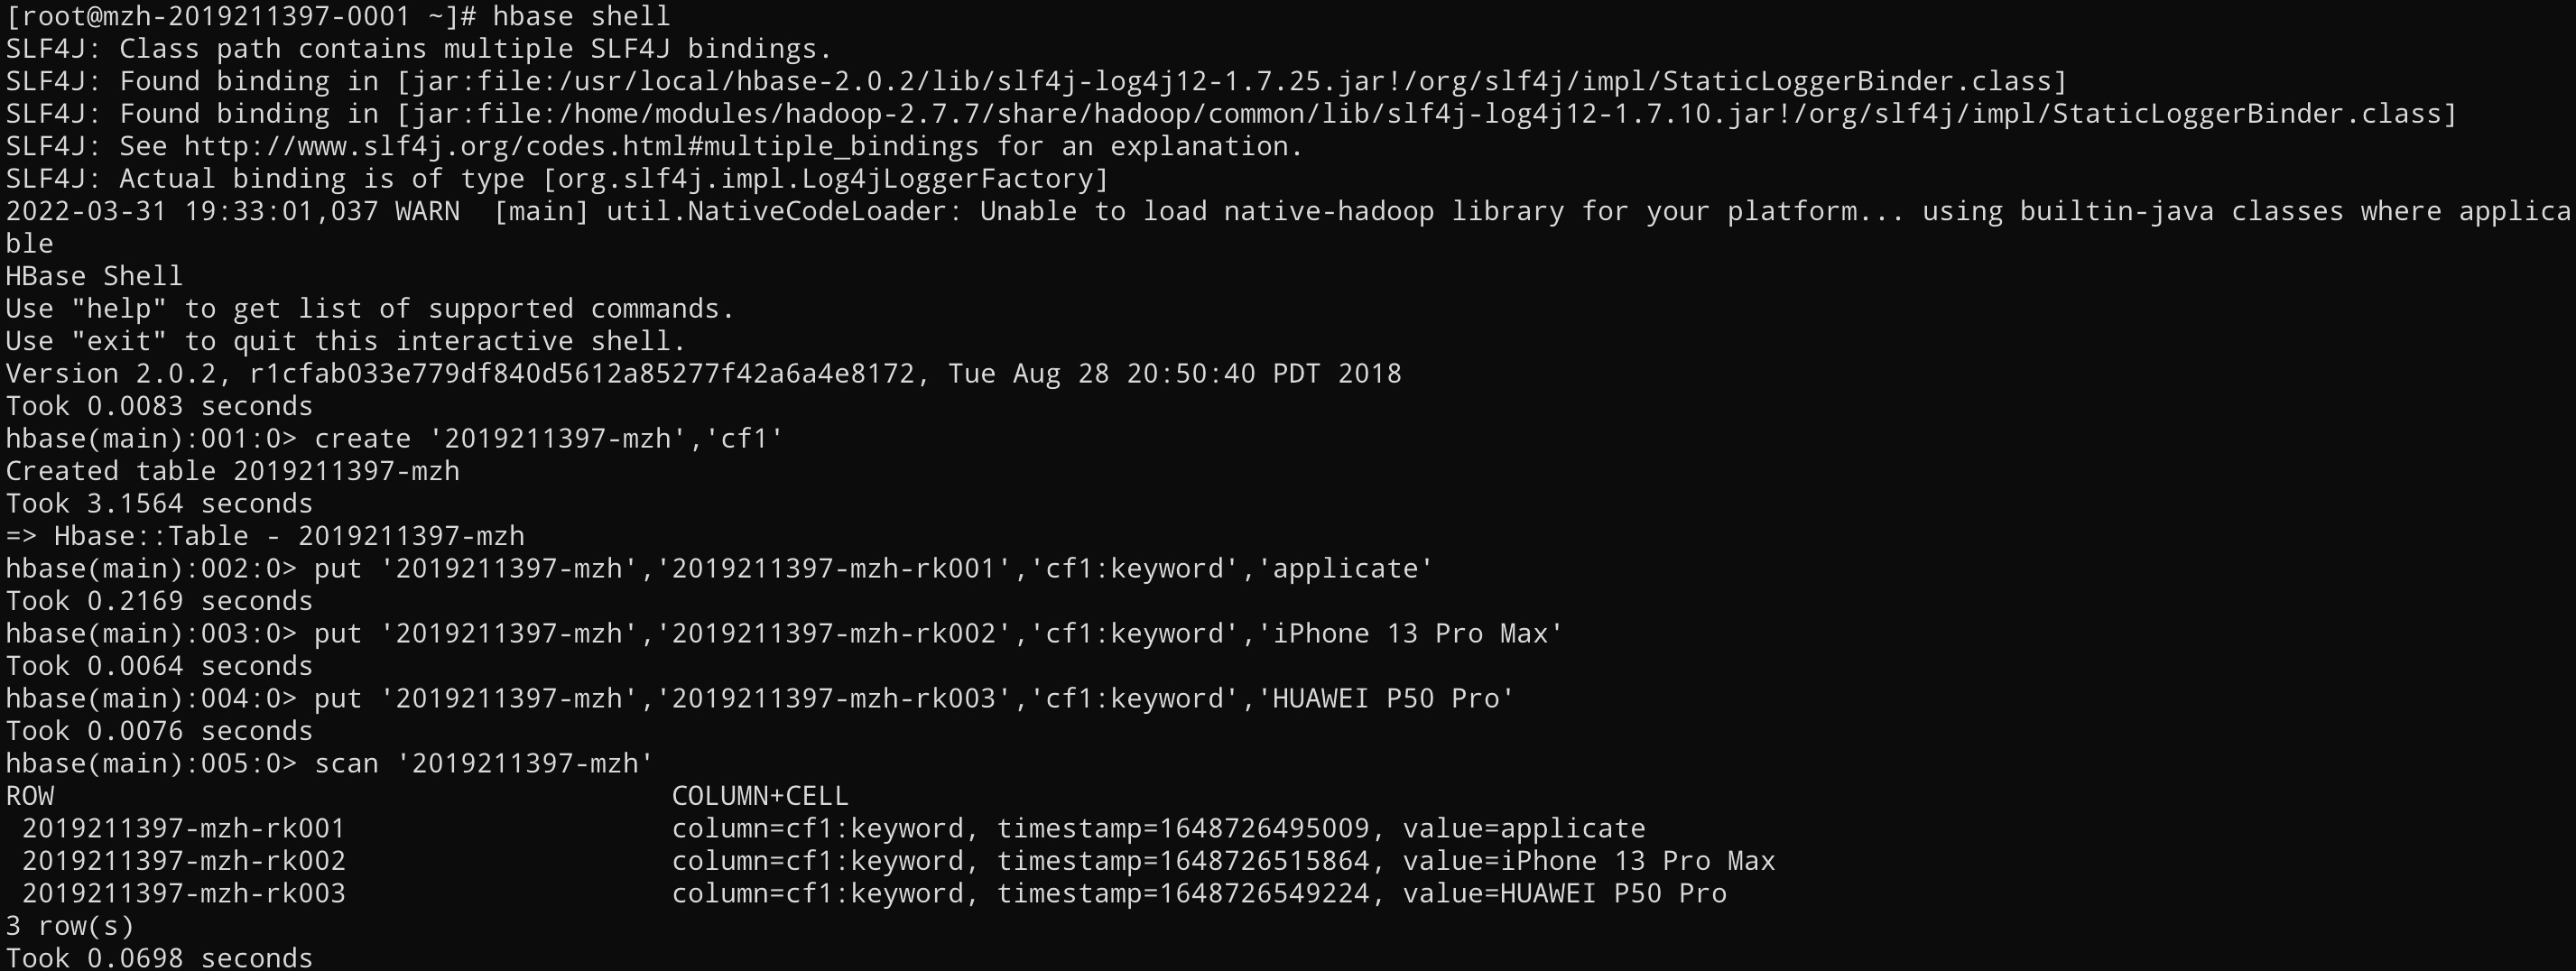
\includegraphics[width=\textwidth]{./images/shell.jpg}
    \caption{HBase Shell操作\label{fig:shell}}
\end{figure}

\paragraph{程序编写}

编写Java代码,其中\mintinline{text}{MemberMapper}类的代码如\figref{fig:mapper}所示。

\begin{figure}[!htb]
    \centering
    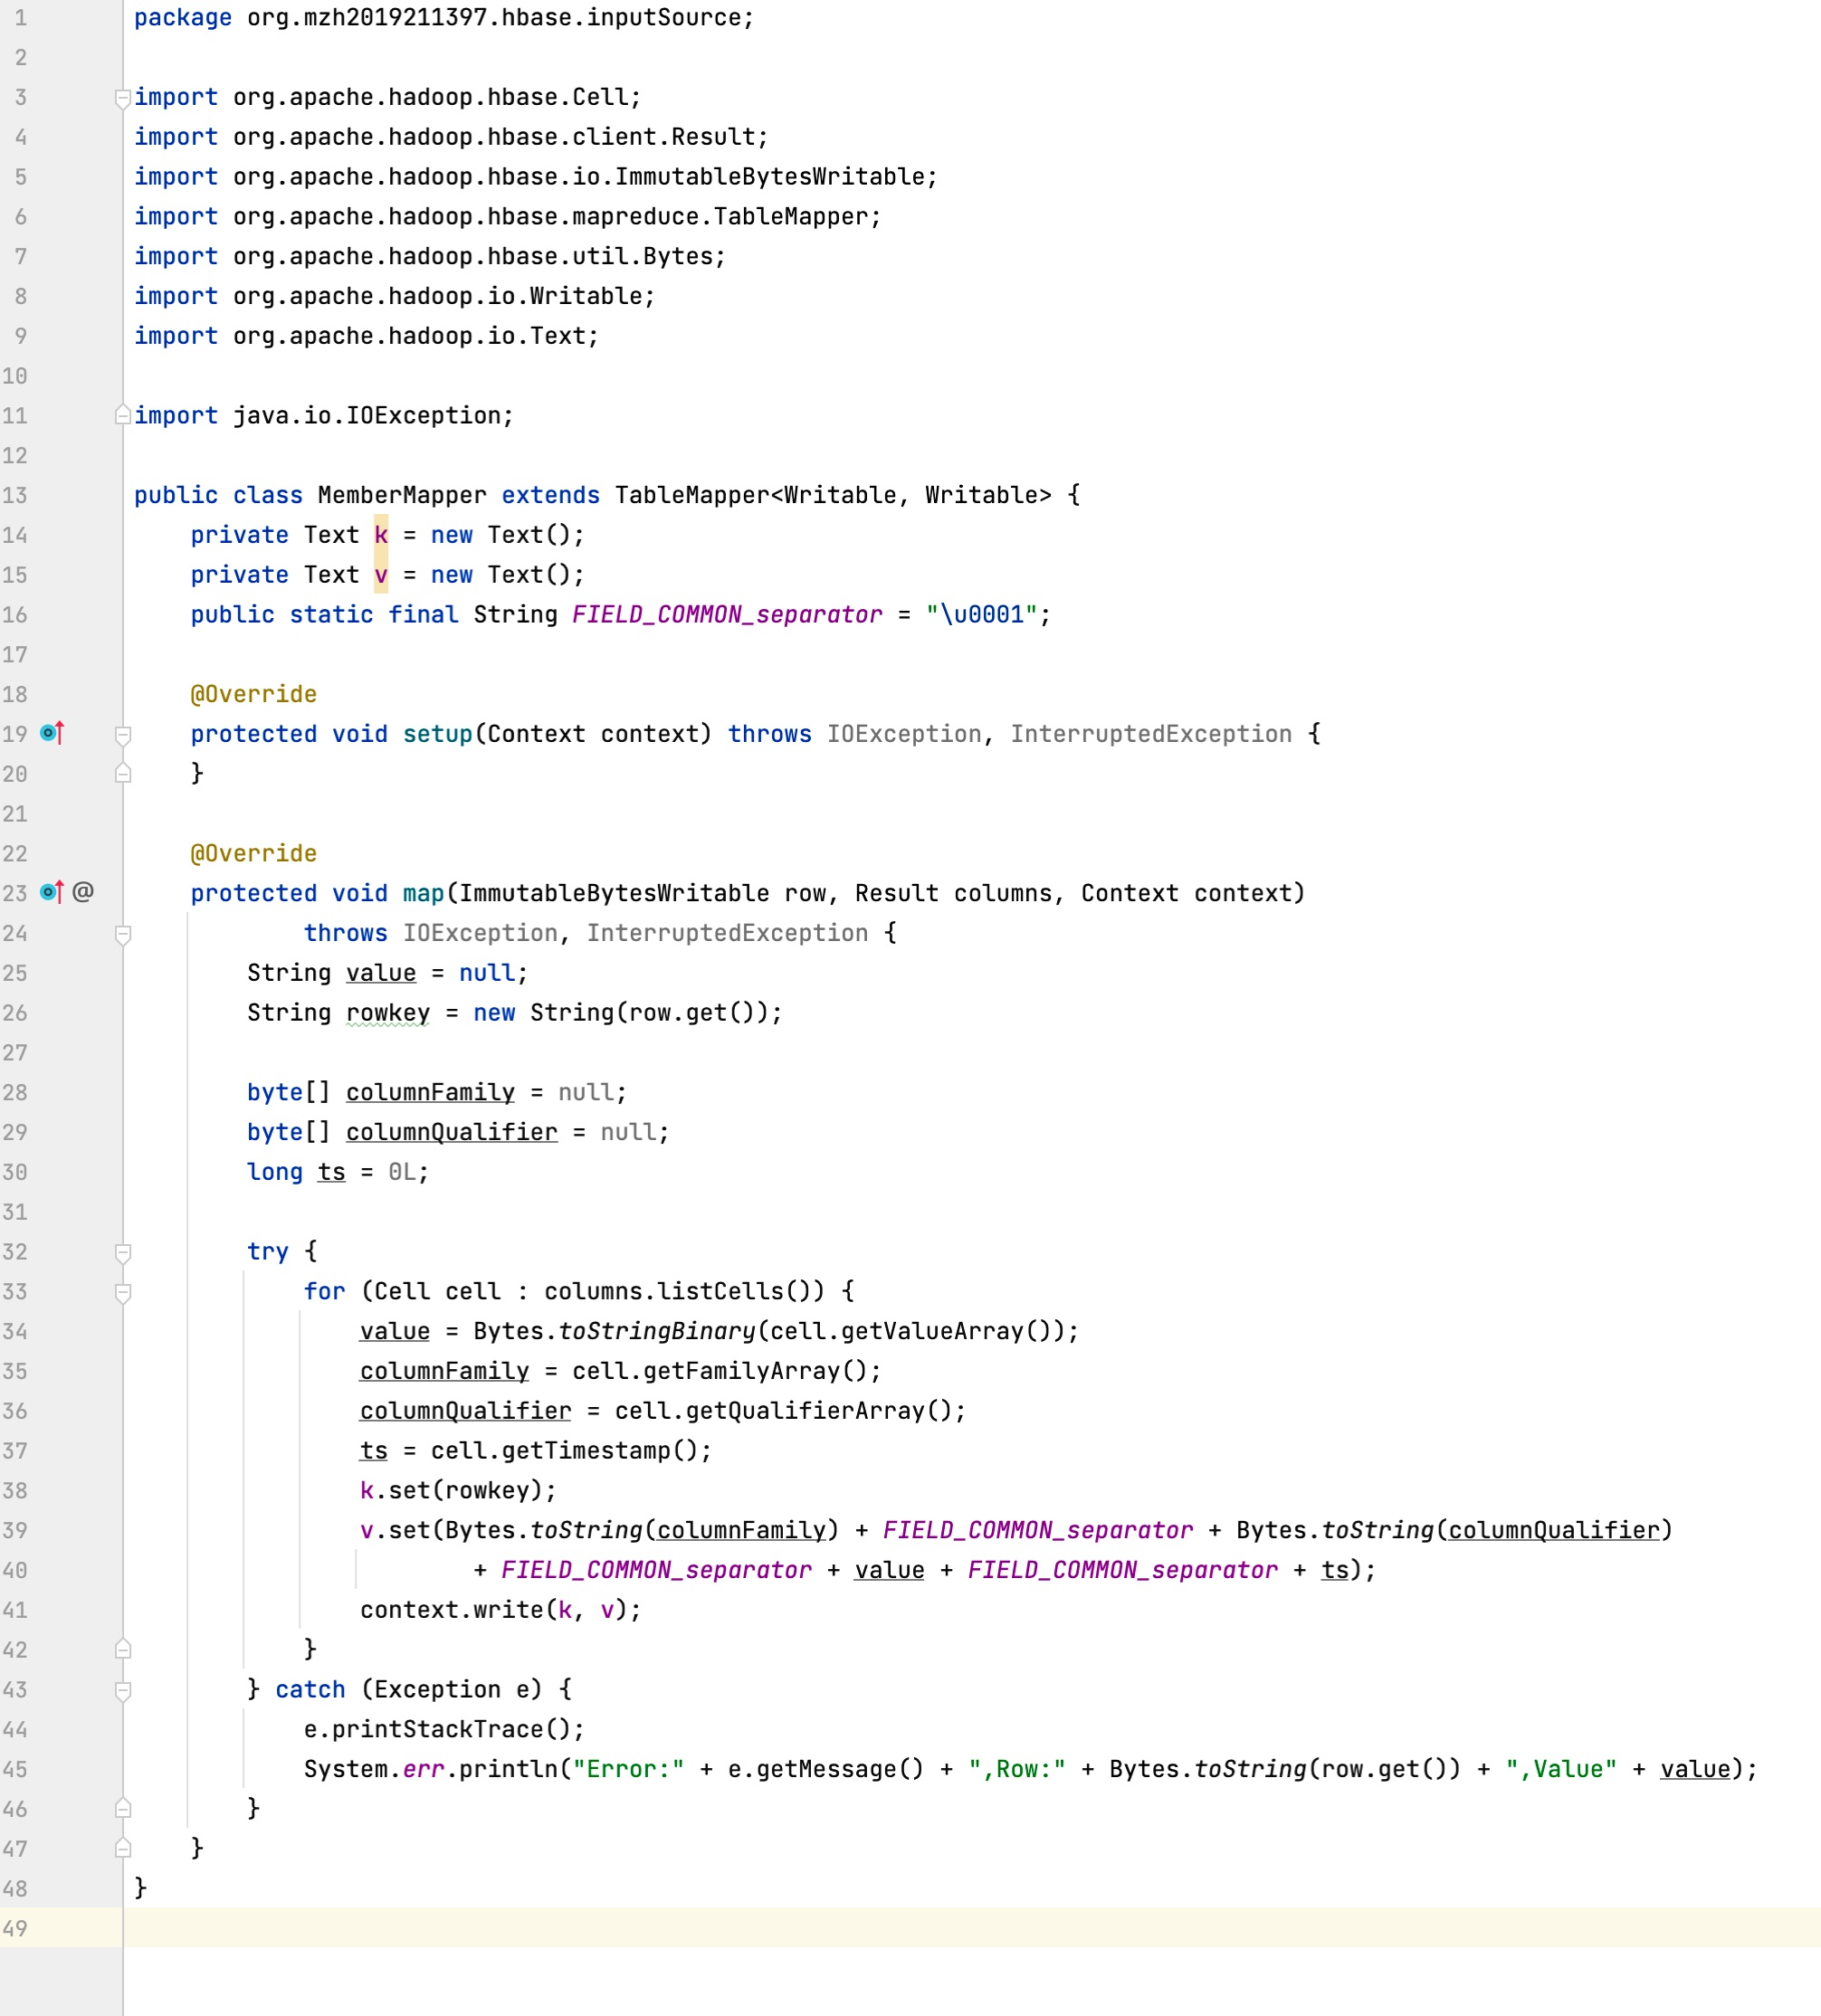
\includegraphics[width=\textwidth]{./images/mapper.jpg}
    \caption{MemberMapper类\label{fig:mapper}}
\end{figure}

该类中的\mintinline{text}{map}方法遍历表的每一行,再遍历该行的每一个单元格,获取每个单元格的值、列族、列限定符、时间戳,将这四者连接起来成为值,以行键作为键,将这样的键值对输出到上下文中。

\paragraph{程序打包和运行}

程序打包后复制到主机上,运行结果如\figref{fig:res}。

\begin{figure}[!htb]
    \centering
    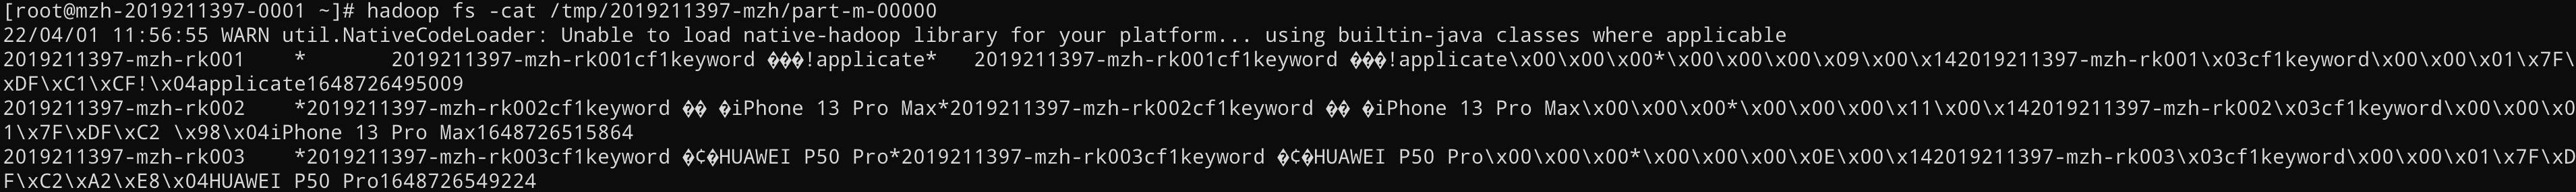
\includegraphics[width=\textwidth]{./images/res.jpg}
    \caption{运行结果\label{fig:res}}
\end{figure}

可见输出了键值对,其中键为行键,值为列族、列限定符、单元格、时间戳的值连接起来。

\section{实验总结}

本次实验中我使用HBase Shell和Java API对HBase进行了简单的操作,使我对HBase和Zookeeper的原理理解更加深刻。

\end{document}
